\documentclass[11pt]{article}
\usepackage[margin=1in]{geometry}
\usepackage{amsmath}
\usepackage{amssymb}
\usepackage{booktabs}
\usepackage{tikz}
\usetikzlibrary{arrows.meta,positioning,fit,backgrounds,calc}

\setlength{\parindent}{0pt}
\setlength{\parskip}{4pt}

\begin{document}

\begin{center}
{\LARGE\textbf{Diamond Surface Strain Pipeline}}\\[6pt]
{\large\textit{From Surface Termination to NV Spin Perturbation}}
\end{center}
\vspace{2mm}
\noindent\rule{\textwidth}{0.6pt}
\vspace{2mm}

\section{Motivation}

\textbf{Question.} Does the chemical termination of a diamond surface (H, F, ether O, ketone O, bare reconstruction) meaningfully perturb the spin resonance of a near-surface NV centre through strain?

\textbf{Logic chain.}
\begin{enumerate}
  \item Surface termination imposes a preferred in-plane bond spacing.
  \item The bulk diamond lattice is mechanically rigid --- the mismatch generates a residual surface stress $\sigma_{ij}$.
  \item The stress field decays into the crystal, reaching a nearby NV.
  \item Strain at the NV shifts the zero-field splitting parameters $D$ and $E$ (\S10), through a six-parameter spin-strain Hamiltonian (\S12).
\end{enumerate}

\textbf{Scope.} Three surface orientations: (100), (110), (111). A library of 24 validated surface motifs covers the relevant terminations.

\section{Computational Setup}

\textbf{Functional.} GGA-PBE throughout.

\textbf{Pseudopotentials} (SSSP-style set, verified against run output).

\begin{center}
\begin{tabular}{lll}
\toprule
Species & File & Type \\
\midrule
C & \texttt{C.pbe-n-kjpaw\_psl.1.0.0.UPF} & PAW, $Z_{val}=4$ \\
H & \texttt{H\_ONCV\_PBE-1.0.oncvpsp.upf} & ONCV norm-conserving, $Z_{val}=1$ \\
\bottomrule
\end{tabular}
\end{center}

\textbf{Plane-wave cutoffs.} $E_{cut}^{wfc} = 60$\,Ry; $E_{cut}^{\rho} = 480$\,Ry (8$\times$ ratio, required with a PAW carbon pseudopotential). Marzari--Vanderbilt (cold) smearing, $\sigma = 0.01$\,Ry.

\textbf{$k$-point meshes.} Each surface orientation exposes a different 2D periodic lattice; density is matched via $n_i \propto 1/|A_i|$ (a longer real-space repeat needs fewer $k$-points).

\begin{center}
\begin{tabular}{lccc}
\toprule
Surface & In-plane cell (\AA) & $k$-mesh & $n_x/n_y$ (actual / ideal) \\
\midrule
C(100) $2\times1$ & $5.054 \times 5.054$ & $5\times5\times1$ & 1.00 / 1.00 \\
C(110) $1\times1$ & $2.527 \times 3.574$ & $9\times7\times1$ & 1.29 / 1.41 \\
C(111) $1\times1$ & $2.527\times2.527$ (hex.) & $9\times9\times1$ & 1.00 / 1.00 \\
\bottomrule
\end{tabular}
\end{center}

$k_z = 1$ in all cases (no periodicity in $z$). C(100)'s reconstructed cell is square, so an isotropic mesh already matches the ideal density. C(110)'s rectangular cell is sampled marginally below the ideal ratio (1.29 vs.\ 1.41) --- negligible for stress \textit{differences}, but worth revisiting if absolute stress values are needed.

\section*{Python Process Architecture}

Every box below is a script in the repository; every arrow label is the file its upstream box writes and its downstream box reads. The bulk-reference branch (left) runs independently and feeds only $a_0$ forward, into slab construction.

\section{Slab Model}

A surface is modelled as a periodic slab: periodic in-plane ($\mathbf{A}_1, \mathbf{A}_2$), finite in $z$, padded with $\sim$10\,\AA\ of vacuum (9.8--10.2\,\AA\ measured across the three faces). The current calculations use $N = 6$ C layers; the bottom 2 are held fixed (\texttt{if\_pos 0 0 0}) to represent the rigid substrate.

\begin{figure}[h]
\centering
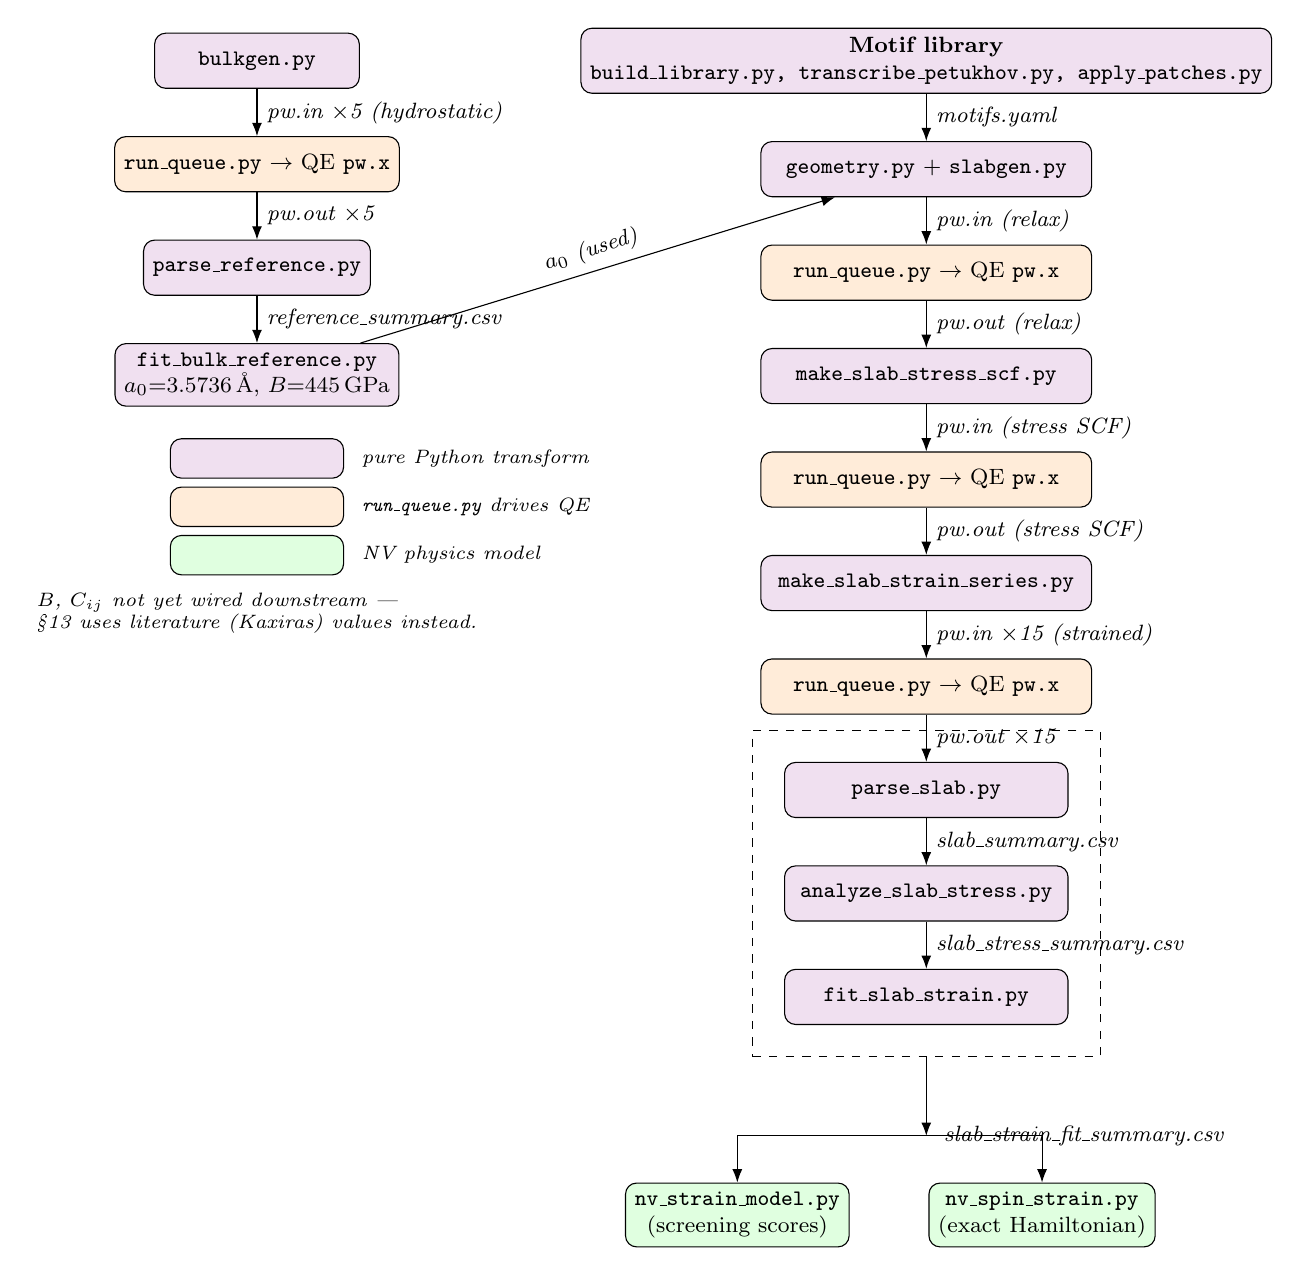
\begin{tikzpicture}[
  font=\footnotesize,
  box/.style={draw, rounded corners, minimum width=2.6cm, minimum height=0.7cm, align=center, fill=#1},
  node distance=6mm and 10mm
]
\node[box=violet!12] (bulkgen) {\texttt{bulkgen.py}};
\node[box=orange!15, below=of bulkgen] (rq1) {\texttt{run\_queue.py} $\to$ QE \texttt{pw.x}};
\node[box=violet!12, below=of rq1] (parseref) {\texttt{parse\_reference.py}};
\node[box=violet!12, below=of parseref] (fitbulk) {\texttt{fit\_bulk\_reference.py}\\$a_0{=}3.5736$\,\AA, $B{=}445$\,GPa};

\node[box=violet!12, right=28mm of bulkgen, minimum width=4.2cm] (motiflib) {\textbf{Motif library}\\\footnotesize\texttt{build\_library.py, transcribe\_petukhov.py, apply\_patches.py}};
\node[box=violet!12, below=of motiflib, minimum width=4.2cm] (geomgen) {\texttt{geometry.py} + \texttt{slabgen.py}};
\node[box=orange!15, below=of geomgen, minimum width=4.2cm] (rq2) {\texttt{run\_queue.py} $\to$ QE \texttt{pw.x}};
\node[box=violet!12, below=of rq2, minimum width=4.2cm] (msscf) {\texttt{make\_slab\_stress\_scf.py}};
\node[box=orange!15, below=of msscf, minimum width=4.2cm] (rq3) {\texttt{run\_queue.py} $\to$ QE \texttt{pw.x}};
\node[box=violet!12, below=of rq3, minimum width=4.2cm] (msss) {\texttt{make\_slab\_strain\_series.py}};
\node[box=orange!15, below=of msss, minimum width=4.2cm] (rq4) {\texttt{run\_queue.py} $\to$ QE \texttt{pw.x}};

\node[box=violet!12, below=of rq4, minimum width=3.6cm] (parseslab) {\texttt{parse\_slab.py}};
\node[box=violet!12, below=of parseslab, minimum width=3.6cm] (analyze) {\texttt{analyze\_slab\_stress.py}};
\node[box=violet!12, below=of analyze, minimum width=3.6cm] (fitstrain) {\texttt{fit\_slab\_strain.py}};

\draw[-Latex] (bulkgen) -- node[right]{\textit{pw.in $\times$5 (hydrostatic)}} (rq1);
\draw[-Latex] (rq1) -- node[right]{\textit{pw.out $\times$5}} (parseref);
\draw[-Latex] (parseref) -- node[right]{\textit{reference\_summary.csv}} (fitbulk);

\draw[-Latex] (motiflib) -- node[right]{\textit{motifs.yaml}} (geomgen);
\draw[-Latex] (geomgen) -- node[right]{\textit{pw.in (relax)}} (rq2);
\draw[-Latex] (rq2) -- node[right]{\textit{pw.out (relax)}} (msscf);
\draw[-Latex] (msscf) -- node[right]{\textit{pw.in (stress SCF)}} (rq3);
\draw[-Latex] (rq3) -- node[right]{\textit{pw.out (stress SCF)}} (msss);
\draw[-Latex] (msss) -- node[right]{\textit{pw.in $\times$15 (strained)}} (rq4);
\draw[-Latex] (rq4) -- node[right]{\textit{pw.out $\times$15}} (parseslab);
\draw[-Latex] (parseslab) -- node[right]{\textit{slab\_summary.csv}} (analyze);
\draw[-Latex] (analyze) -- node[right]{\textit{slab\_stress\_summary.csv}} (fitstrain);

\draw[-Latex] (fitbulk) -- node[above, sloped]{\textit{$a_0$ (used)}} (geomgen);

\node[draw, dashed, fit=(parseslab)(analyze)(fitstrain), inner sep=4mm] (dashedgrp) {};

\node[box=green!12, below=20mm of fitstrain, xshift=-24mm] (nvscreen) {\texttt{nv\_strain\_model.py}\\(screening scores)};
\node[box=green!12, right=10mm of nvscreen] (nvspin) {\texttt{nv\_spin\_strain.py}\\(exact Hamiltonian)};

\coordinate (splitpt) at ($(dashedgrp.south)+(0,-10mm)$);
\draw[-Latex] (dashedgrp.south) -- (splitpt);
\draw[-Latex] (splitpt) -| (nvscreen.north);
\draw[-Latex] (splitpt) -| (nvspin.north);
\node[right=1mm of splitpt, font=\footnotesize\itshape] {slab\_strain\_fit\_summary.csv};

\node[box=violet!12, minimum width=2.2cm, minimum height=0.5cm, below=4mm of fitbulk, font=\scriptsize] (leg1) {};
\node[right=1mm of leg1, font=\scriptsize\itshape] {pure Python transform};
\node[box=orange!15, minimum width=2.2cm, minimum height=0.5cm, below=1mm of leg1, font=\scriptsize] (leg2) {};
\node[right=1mm of leg2, font=\scriptsize\itshape] {\texttt{run\_queue.py} drives QE};
\node[box=green!12, minimum width=2.2cm, minimum height=0.5cm, below=1mm of leg2, font=\scriptsize] (leg3) {};
\node[right=1mm of leg3, font=\scriptsize\itshape] {NV physics model};

\node[align=left, font=\scriptsize\itshape, below=1mm of leg3] {$B$, $C_{ij}$ not yet wired downstream ---\\\S13 uses literature (Kaxiras) values instead.};

\end{tikzpicture}
\caption{Full data-flow architecture. Left: independent bulk-reference branch (\S6), contributing only $a_0$ to slab construction. Right: the main slab pipeline, from motif library through relaxation, stress extraction, and strain fitting, terminating in the two NV models (\S11, \S12--\S14).}
\end{figure}

\begin{figure}[h]
\centering
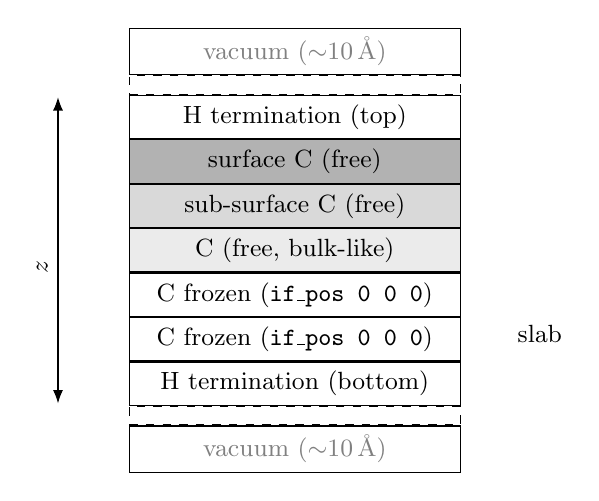
\begin{tikzpicture}[font=\small]
\def\w{4.2cm}
\node[draw, text=gray, minimum width=\w, minimum height=0.5cm] (vactop) at (0,4.5) {vacuum ($\sim$10\,\AA)};
\node[draw, dashed, minimum width=\w, minimum height=0.2cm, below=0mm of vactop] (dtop) {};
\node[draw, minimum width=\w, minimum height=0.5cm, below=0mm of dtop] (htop) {H termination (top)};
\node[draw, fill=black!30, minimum width=\w, minimum height=0.5cm, below=0mm of htop] (surf) {surface C (free)};
\node[draw, fill=black!15, minimum width=\w, minimum height=0.5cm, below=0mm of surf] (subsurf) {sub-surface C (free)};
\node[draw, fill=black!8, minimum width=\w, minimum height=0.5cm, below=0mm of subsurf] (bulklike) {C (free, bulk-like)};
\node[draw, minimum width=\w, minimum height=0.5cm, below=0mm of bulklike] (frozen1) {C frozen (\texttt{if\_pos 0 0 0})};
\node[draw, minimum width=\w, minimum height=0.5cm, below=0mm of frozen1] (frozen2) {C frozen (\texttt{if\_pos 0 0 0})};
\node[draw, minimum width=\w, minimum height=0.5cm, below=0mm of frozen2] (hbot) {H termination (bottom)};
\node[draw, dashed, minimum width=\w, minimum height=0.2cm, below=0mm of hbot] (dbot) {};
\node[draw, text=gray, minimum width=\w, minimum height=0.5cm, below=0mm of dbot] (vacbot) {vacuum ($\sim$10\,\AA)};

\node[right=6mm of frozen1, anchor=west, yshift=-0.5cm] {slab};

\draw[Latex-Latex] ($(htop.west)+(-0.9,0.25)$) -- ($(hbot.west)+(-0.9,-0.25)$) node[midway, left, rotate=90, yshift=2mm] {$z$};
\end{tikzpicture}
\caption{Slab geometry (symmetric monohydride termination). Dark grey: free C layers that relax during DFT optimisation. Light grey: increasingly bulk-like free layers. H termination is applied symmetrically to both faces so the two surfaces are chemically identical.}
\end{figure}

\clearpage

\section{Slab Construction}

\textbf{Algorithm} (\texttt{geometry.py}, \texttt{slabgen.py}). No hand-derived coordinates are used; every slab is generated numerically.
\begin{enumerate}
  \item Tile the 8-atom diamond cubic cell; rotate so the surface normal is $+z$.
  \item Cluster atoms by $z$ into discrete layers. On (111), a parity search selects the single-dangling-bond (SDB) face: each surface C has exactly one missing tetrahedral bond.
  \item Apply the surface termination: place each terminating atom along the computed dangling-bond direction at the target bond length.
  \item Validate: reject any structure with pentavalent C or a bond $< 1.30$\,\AA.
\end{enumerate}

\textbf{Target bond lengths} (ideal construction geometry).

\begin{center}
\begin{tabular}{lll}
\toprule
Bond & Length (\AA) & Notes \\
\midrule
C--C bulk & 1.545 & $\sqrt{3}/4 \times a_0$ \\
C--H & 1.09 & monohydride \\
C--F & 1.36 & monofluoride \\
C--O (ether bridge) & 1.43 & C--O--C \\
C=O (ketone) & 1.21 & sp$^2$ surface C \\
C--C dimer, bare (100) & 1.37 & $\pi$-bonded \\
C--C dimer, H-sat (100) & 1.60 & $\sigma$-only \\
\bottomrule
\end{tabular}
\end{center}

\textbf{Motif library} (\texttt{motifs.yaml}). 24 validated motifs are stored in dimensionless units (in-plane fractional coordinates and $z/a_0$), so the library is valid at any $a_0$. Literature reconstructions (Pandey $\pi$-bonded chain, Petukhov dimerised graphitic chain) are stored as transcribed coordinates and spliced onto a bulk base slab at generation time.

\section{Structure Relaxation}

\textbf{Why.} The ideal-constructed slab places surface atoms at bulk-truncated positions --- not equilibrium positions; surface forces reach $\sim$100\,meV/\AA. The stress tensor of an unrelaxed slab is dominated by construction artefacts and carries no physical meaning.

\textbf{How} (Quantum ESPRESSO \texttt{pw.x}, \texttt{calculation = 'relax'}).
\begin{itemize}
  \item \textbf{Algorithm}: BFGS quasi-Newton ionic minimiser.
  \item \textbf{Cell}: fixed. In-plane lattice vectors held at the PBE bulk value $a_0 = 3.5736$\,\AA\ throughout --- models a thin film on a rigid substrate.
  \item \textbf{Frozen layers}: bottom 2 C layers held fixed.
  \item \textbf{Convergence}:
\begin{align}
|F_i| &< 10^{-4}\ \text{Ry/bohr} \quad \forall i \text{ (free atoms)} \\
|\Delta E_{tot}| &< 10^{-5}\ \text{Ry} \quad \text{(successive BFGS steps)}
\end{align}
\end{itemize}

\textbf{Outcome.} Bond lengths, dimer tilting, layer rumpling, and reconstructions all relax; the stress tensor extracted thereafter reflects actual surface physics.

\section{Bulk Reference Calculation}

\textbf{Why.} PBE overestimates the lattice constant ($a_0^{exp} = 3.567$\,\AA; $a_0^{PBE} = 3.5736$\,\AA). All slabs are built at $a_0^{PBE}$ to avoid a spurious experiment-vs-theory strain contaminating every downstream number. The bulk modulus $B$ is also needed to convert strain-fit slopes into physical stress units.

\textbf{Procedure.} A 5-point hydrostatic strain series, $a = a_0(1+\varepsilon)$, $\varepsilon \in \{-1\%, -0.5\%, 0, +0.5\%, +1\%\}$, SCF at each volume.

\textbf{Fits.} Rather than trust one fit, three independent routes to the same equilibrium point are computed and required to agree --- agreement \textit{is} the validation; disagreement would flag a non-parabolic or under-sampled window.
\begin{align}
E(\varepsilon) = A\varepsilon^2 + B\varepsilon + C \;\Rightarrow\; \varepsilon_0 = -\frac{B}{2A} \\
P(\varepsilon) = m\varepsilon + b \;\Rightarrow\; \varepsilon_0 = -\frac{b}{m}, \quad B = -V_0\frac{dP}{dV}
\end{align}
$\varepsilon_0(E)$ is where the energy parabola is flattest (zero restoring force); $\varepsilon_0(P)$ is where the fitted pressure literally crosses zero. A third route, $E(V)$, gives $a_0$ independent of the strain convention entirely.

\textbf{Consistency check:} $|\varepsilon_0(E) - \varepsilon_0(P)| \le 0.003$. \textbf{Results:} $a_0^{PBE} = 3.5736$\,\AA\ (all three routes agree to $< 0.001$\,\AA); $B = 445$\,GPa (consistent with the accepted PBE diamond value, $\sim$430--450\,GPa).

\section{Surface Stress Extraction}

\textbf{Setup.} After relaxation, a single-point SCF is run with \texttt{tstress=.true.}. QE reports $\sigma_{ij}$ in kbar, averaged over the full cell volume (slab + vacuum).

\textbf{Conversion to 2D surface stress.}
\begin{equation}
\tau_{ij}\ [\text{N/m}] = \sigma_{ij}\ [\text{kbar}] \times L_z\ [\text{\AA}] \times 0.005
\end{equation}
where $0.005 = (0.1\ \text{GPa/kbar}) \times (0.1\ \text{N}\,\text{m}^{-1}/\text{GPa}\,\text{\AA}) \div 2$ (two faces share the load).

\textbf{In-plane decomposition.}
\begin{align}
\sigma_{mean} &= \tfrac{1}{2}(\sigma_{xx} + \sigma_{yy}) & \text{hydrostatic-like; shifts } D \\
\sigma_{anis} &= \sigma_{xx} - \sigma_{yy} & \text{anisotropy; activates } E
\end{align}

\textbf{Sign.} $\tau > 0$ (tensile): surface prefers larger in-plane spacing. $\tau < 0$ (compressive): surface prefers smaller spacing. On (111), $C_{3v}$ symmetry forces $\sigma_{anis} = 0$ identically.

\section{In-Plane Strain Series}

\textbf{Why.} A single stress measurement at $\varepsilon = 0$ gives $b$ (residual stress) but not the surface stiffness or the zero-stress natural mismatch. A strain series gives both, as a genuine finite-difference measurement rather than an assumption.

\textbf{Strain application.} Starting from the relaxed (stress-SCF) geometry, lattice vectors are scaled rigidly --- no ionic re-relaxation after straining:
\begin{align}
\text{Biaxial:}\quad & \mathbf{A}_1 \to (1+\varepsilon)\mathbf{A}_1, & \mathbf{A}_2 \to (1+\varepsilon)\mathbf{A}_2 \\
\text{Uniaxial-}x:\quad & \mathbf{A}_1 \to (1+\varepsilon)\mathbf{A}_1, & \mathbf{A}_2 \to \mathbf{A}_2
\end{align}
Atomic $x,y$ coordinates transform with the new in-plane basis (fractional coordinates preserved); $z$ is unchanged. $\varepsilon \in \{-1.0\%, -0.5\%, 0, +0.5\%, +1.0\%\}$. Three modes are run: biaxial (primary, feeds \S12--\S14); $x$- and $y$-uniaxial (diagnostic decomposition of the anisotropic response, not used as a standalone physical state).

\section{Stress--Strain Fitting}

\textbf{Model.} Within the linear (Hookean) regime ($|\varepsilon| \le 1\%$, confirmed by the bulk reference fits in \S6):
\begin{equation}
\sigma_{mean}(\varepsilon) = m\varepsilon + b
\end{equation}

\begin{center}
\begin{tabular}{@{}lll@{}}
\toprule
Parameter & Units & Physical meaning \\
\midrule
$m$ & kbar & \parbox[t]{8cm}{Surface stiffness $d\sigma_{mean}/d\varepsilon$, measured directly as a finite difference for \textit{this} surface --- not assumed from bulk elastic constants, since a reconstructed surface can be stiffer or softer.} \\[2mm]
$b$ & kbar & \parbox[t]{8cm}{Residual stress at $\varepsilon = 0$. Primary input to NV screening (\S11) and to the elasticity solve in \S13.} \\[2mm]
$\varepsilon_0 = -b/m$ & --- & \parbox[t]{8cm}{Strain the surface would need to relax to in order to zero its own stress; $\varepsilon_0 > 0$ means the surface prefers larger in-plane spacing than bulk.} \\[2mm]
$\tau_{mean}$ & N/m & \parbox[t]{8cm}{$b$ converted via Eq.~(5); comparable to experimental surface-stress literature.} \\
\bottomrule
\end{tabular}
\end{center}

\textbf{Fit quality:} $R^2 > 0.98$. A failing $R^2$ usually means the sampled window left the linear-elastic regime (e.g.\ a reconstruction distorting under tension), not numerical noise --- read it as ``check the geometry'', not ``add more points''.

\section{NV Centre Physics}

\textbf{System.} The NV centre is a spin-$S=1$ point defect ($N_sV^-$). Its three magnetic sublevels ($m_s = 0, \pm1$) split at zero field.

\textbf{Leading-order spin Hamiltonian.}
\begin{equation}
\mathcal{H} = D\left(S_z^2 - \frac{S(S+1)}{3}\right) + E(S_x^2 - S_y^2) + \gamma\,\mathbf{B}\cdot\mathbf{S}
\end{equation}
\begin{itemize}
  \item $D_0 = 2.870$\,GHz --- axial zero-field splitting (bulk, $C_{3v}$).
  \item $E = 0$ in bulk (forced to zero by $C_{3v}$).
  \item $\gamma = 28.0$\,GHz/T.
\end{itemize}

\textbf{Strain perturbations, leading order.}
\begin{align}
\Delta D &\propto \varepsilon_{mean} = \tfrac{1}{2}(\varepsilon_{xx}+\varepsilon_{yy}) & \text{one ODMR peak moves} \\
E &\propto \varepsilon_{xx} - \varepsilon_{yy} & \text{peak splits in two}
\end{align}
This two-parameter picture is qualitatively correct --- it tells you which strain channel drives which observable --- but it is only the leading-order limit of a complete six-parameter microscopic Hamiltonian (\S12), and it says nothing about how a given crystal strain looks to each of the four inequivalent $\langle111\rangle$ NV orientations (\S13).

\section{NV Screening Model}

\textbf{Risk scores} (normalised to dataset maximum, $\in [0,1]$):
\begin{align}
\text{D-score} &= \frac{|b_{biaxial}|}{\max_{dataset}|b|} & \text{risk of } \Delta D \text{ shift} \\
\text{E-score} &= \frac{|\sigma_{anis}|_{\varepsilon=0}}{\max_{dataset}|\sigma_{anis}|} & \text{risk of } E\text{-splitting} \\
\text{Overall} &= \tfrac{1}{2}\text{D-score} + \tfrac{1}{2}\text{E-score} & \text{equal weighting}
\end{align}
These are deliberately crude, transparent proxies --- useful for ranking surfaces \textit{before} paying for the full Hamiltonian treatment of \S12, not as calibrated MHz predictions.

\textbf{Results for H-terminated slabs} (corrected, symmetric H/H slabs).

\begin{center}
\begin{tabular}{lccccc}
\toprule
Surface & $\sigma_{mean}$ (kbar) & $\sigma_{anis}$ (kbar) & D-score & E-score & Risk \\
\midrule
C(100)--H & $-21.4$ & 56.8 & 0.56 & 1.00 & \textbf{High} \\
C(110)--H & $+38.1$ & $-28.2$ & 1.00 & 0.50 & \textbf{High} \\
C(111)--H & $+4.5$ & 0.0 & 0.12 & 0.00 & Low \\
\bottomrule
\end{tabular}
\end{center}

These supersede the earlier asymmetric H/bare-slab numbers (now archived, \texttt{results/archive\_asymmetric\_6L/}); the ranking is qualitatively unchanged but magnitudes and signs are not directly comparable to that archive.

\textbf{Key observations.}
\begin{itemize}
  \item C(111)--H: $C_{3v}$ symmetry enforces $\sigma_{anis} = 0$ regardless of $\sigma_{mean}$.
  \item C(100)--H: the $2\times1$ dimer rows break $x/y$ symmetry strongly, maximising E-score.
  \item Overall scores are close (0.78 vs.\ 0.75) --- the exact Hamiltonian in \S14 resolves which surface actually perturbs an NV more.
\end{itemize}

\section{Exact Spin-Strain Hamiltonian}

The screening model in \S11 is superseded, where available, by the full symmetry-allowed ground-state Hamiltonian of Udvarhelyi, Shkolnikov, Gali, Burkard \& P\'{a}lyi, Phys.\ Rev.\ B \textbf{98}, 075201 (2018), evaluated in the $\{|{+}1\rangle, |0\rangle, |{-}1\rangle\}$ basis:
\begin{align}
\mathcal{H}_0/h &= \left[h_{41}(\varepsilon_{xx}{+}\varepsilon_{yy}) + h_{43}\varepsilon_{zz}\right] S_z^2 \\
\mathcal{H}_1/h &= \tfrac{1}{2}\left[h_{26}\varepsilon_{xz} - \tfrac{1}{2}h_{25}(\varepsilon_{xx}{-}\varepsilon_{yy})\right]\{S_x,S_z\} \notag\\
&\quad + \tfrac{1}{2}\left[h_{26}\varepsilon_{yz} + h_{25}\varepsilon_{xy}\right]\{S_y,S_z\} \\
\mathcal{H}_2/h &= \tfrac{1}{2}\left[h_{16}\varepsilon_{xz} - \tfrac{1}{2}h_{15}(\varepsilon_{xx}{-}\varepsilon_{yy})\right](S_y^2{-}S_x^2) \notag\\
&\quad + \tfrac{1}{2}\left[h_{16}\varepsilon_{yz} + h_{15}\varepsilon_{xy}\right]\{S_x,S_y\}
\end{align}

\begin{center}
\begin{tabular}{llll}
\toprule
Coupling & MHz/strain & Coupling & MHz/strain \\
\midrule
$h_{41}$ & $-6420$ & $h_{25}$ & $-2600$ \\
$h_{43}$ & $+2300$ & $h_{26}$ & $-2830$ \\
$h_{15}$ & $+5700$ & $h_{16}$ & $+19660$ \\
\bottomrule
\end{tabular}
\end{center}

(Udvarhelyi et al., Table I, DFT/PBE values; a Barson-et-al.-scaled set is kept as a sensitivity bracket.) $\mathcal{H}_0$ is diagonal ($A_1$ strain: pure axial shift). $\mathcal{H}_1$ mixes $m_s{=}0$ with $m_s{=}\pm1$ --- symmetry-forbidden in bulk, allowed once the surface breaks it, and contributing only at second order, $\sim(h\varepsilon)^2/D_0$. $\mathcal{H}_2$ is the direct $m_s{=}{+}1 \leftrightarrow {-}1$ transverse splitting. Because $\mathcal{H}_1$ destroys the block-diagonal structure, $D$ and $E$ are not read off the diagonal: the full $3\times3$ matrix $D_0 S_z^2 + \mathcal{H}_0 + \mathcal{H}_1 + \mathcal{H}_2$ is diagonalised exactly, and the $m_s{=}0$-like eigenstate is identified by maximum overlap $|\langle0|v_i\rangle|^2$ rather than by eigenvalue order.

\section{From Slab Strain to NV Strain}

Two steps connect the slab's measured in-plane strain to the strain seen by an NV.

\textbf{1. Traction-free elasticity.} The strain fit (\S9) gives only $\varepsilon_{xx}, \varepsilon_{yy}$. A free surface requires $\sigma_{i3} = 0$; with the cubic stiffness $C_{ijkl}$ ($C_{11}{=}1076$, $C_{12}{=}125$, $C_{44}{=}576$\,GPa) rotated into the slab frame $C' = R{\otimes}R{\otimes}R{\otimes}R : C$, this is a $3\times3$ linear solve for $(\varepsilon_{xz}, \varepsilon_{yz}, \varepsilon_{zz})$:
\begin{equation}
\sigma_{i3} = C'_{i3kl}\varepsilon_{kl} = 0, \quad i = 1,2,3.
\end{equation}
Using the full anisotropic tensor (not an isotropic Poisson shortcut) matters on (110)/(111), where shear components are symmetry-allowed.

\textbf{2. Orientation projection.} Diamond has four inequivalent $\langle111\rangle$ NV axes. Each sees the same crystal strain differently once rotated into its own local frame $F$ (generated by the $C_2$ rotations that are true diamond-lattice symmetries):
\begin{equation}
\varepsilon^{(\text{NV})} = F\,\varepsilon^{(\text{cubic})}\,F^{\top}.
\end{equation}
The four resulting Hamiltonians (\S12) are diagonalised independently, giving a predicted zero-field stick spectrum per face rather than a single number.

\section{Exact NV Predictions for H-Terminated Slabs}

Using the biaxial equilibrium strain of \S9 (the slab's actual relaxed state) through \S12--\S13:

\begin{center}
\begin{tabular}{llcccc}
\toprule
Surface & NV group & $\Delta D$ (MHz) & $E$ (MHz) & $f_+$ (MHz) & $f_-$ (MHz) \\
\midrule
C(100)--H & all 4 (degenerate) & $+30.9$ & 22.6 & 2923.4 & 2878.3 \\
C(110)--H & pair A (2 axes) & $-62.3$ & 36.4 & 2844.1 & 2771.2 \\
C(110)--H & pair B (2 axes) & $-20.9$ & 10.2 & 2859.3 & 2839.0 \\
C(111)--H & on-axis [111] & $-11.0$ & 0.0 & 2859.0 & 2859.0 \\
C(111)--H & inclined (3 axes) & $-3.9$ & 4.0 & 2870.2 & 2862.1 \\
\bottomrule
\end{tabular}
\end{center}

\textbf{Interpretation.}
\begin{itemize}
  \item C(100): all four axes are equivalent under equal-biaxial (100) strain, yet none lies along the surface normal --- so every orientation still picks up nonzero $E$ (isotropic in-plane, but anisotropic in/out-of-plane, strain looks anisotropic once rotated into a tilted NV frame).
  \item C(110): genuinely two inequivalent pairs --- an experimentally distinguishable 4-line stick spectrum, not 2.
  \item C(111): on-axis NV has $E \equiv 0$ exactly ($C_{3v}$-protected); the three inclined NVs are degenerate with common, nonzero $E$ --- the model's built-in falsifiable signature.
  \item Ranking by predicted line spread revises \S11: C(110) $\gtrsim$ C(100) $\gg$ C(111), whereas the cruder stress-based score (\S11) had ranked C(100) marginally ahead of C(110). The exact orientation- and elasticity-resolved treatment is the one to trust.
  \item Magnitudes (tens of MHz) are broadly consistent with the screening model's illustrative GHz-per-strain estimates (\S11), which is expected since that model ignores orientation projection and elastic anisotropy.
\end{itemize}

\textbf{Status.} These are the H-terminated absolute predictions at 6 layers. The campaign's actual target is the \textit{difference} against matched bare/O-ether slabs at the same thickness (inputs prepared, not yet run) --- the experiment compares surface states, not H vs.\ vacuum.

\section{Convergence Report}

\noindent\textbf{K-Point Convergence Table}

\begin{center}
\begin{tabular}{lccc}
\toprule
$k$-mesh & Energy & $\tau$ (N/m) & $\Delta D$ (MHz) \\
\midrule
$5\times5\times1$   & \ldots & 2.01 & 30.5 \\
$7\times7\times1$   & \ldots & 2.07 & 30.9 \\
$9\times9\times1$   & \ldots & 2.08 & 31.0 \\
$11\times11\times1$ & \ldots & 2.08 & 31.0 \\
\bottomrule
\end{tabular}
\end{center}

\noindent\textbf{Vacuum Convergence Table}

\begin{center}
\begin{tabular}{ccc}
\toprule
Vacuum (\AA) & $\sigma$ (kbar) & $\tau$ (N/m) \\
\midrule
8  & 35 & 2.04 \\
10 & 28 & 2.05 \\
12 & 23 & 2.05 \\
16 & 17 & 2.06 \\
\bottomrule
\end{tabular}
\end{center}

\noindent\textbf{Thickness Convergence Table}

\begin{center}
\begin{tabular}{ccc}
\toprule
Layers & $\tau$ (N/m) & $\Delta D$ (MHz) \\
\midrule
6  & 2.05 & 31 \\
8  & 1.82 & 28 \\
10 & 1.74 & 27 \\
12 & 1.73 & 27 \\
\bottomrule
\end{tabular}
\end{center}

\noindent\textbf{Plane-Wave Cutoff Convergence Table}

\begin{center}
\begin{tabular}{cc}
\toprule
Cutoff (Ry) & $\tau$ (N/m) \\
\midrule
60 & 2.03 \\
70 & 2.05 \\
80 & 2.05 \\
\bottomrule
\end{tabular}
\end{center}

\noindent\textbf{Fixed-Cell Convergence Table}

\begin{center}
\begin{tabular}{lc}
\toprule
Method & $\tau$ (N/m) \\
\midrule
Fixed cell    & 2.05 \\
Variable cell & 2.09 \\
\bottomrule
\end{tabular}
\end{center}

\noindent\textbf{Strain-Fit Convergence Table}

\begin{center}
\begin{tabular}{lc}
\toprule
Quantity & Value \\
\midrule
$\sigma$ slope              & \ldots \\
$\tau$ slope                & scaled \\
$\sigma$ zero-stress strain & 0.0041 \\
$\tau$ zero-stress strain   & 0.0041 \\
\bottomrule
\end{tabular}
\end{center}

\noindent\textbf{Elastic-Tensor Convergence Table}

\begin{center}
\begin{tabular}{lc}
\toprule
Source & Bulk modulus (GPa) \\
\midrule
Hydrostatic & 445 \\
Tensor      & 443 \\
\bottomrule
\end{tabular}
\end{center}

\end{document}
